\chapter{Introduction}


\section{Context}

\subsection{CERN}
CERN (Conseil Europ\'{e}en pour la Recherche Nucl\'{e}aire or European Organization for Nuclear Research)\cite{CERN}, founded in 1952, is the biggest research center in the area of particle physics. It is located in the French-Swiss border, near Geneva. Even though CERN directly employs around 2400 people, more than 10000 scientist from around 113 countries have visited CERN to deepen their research. As an example of its contributions to science, recently, in July of 2012, CERN announced that two different experiments (ATLAS and CMS) confirmed the existence of the particle named Higgs Boson, which lead to the award of the Nobel Prize to Peter Higgs and Fran\c{c}ois Englert.

Even though the main focus of CERN relies on the study of particle physics, the strong research environment has lead to important advances in several different areas, and one of the main inventions that CERN has contributed to the world is the Web. Tim Berners-Lee, in 1989, proposed a solution\cite{web_proposal} to the increasing problem of keeping track all the information related to the different experiments held at CERN, through a hypertext system. 

\subsection{CDS Invenio}
CDS\cite{CDS1} (CERN Document Server) Invenio is the integrated digital library system developed and used at CERN\cite{CDS2}. To the date, it contains more than one million records and more than 400000 full-text documents. It provides tools to manage the complete workflow of a document taking care of the submission, annotation, edition, storage, searching, retrieval, displaying among other phases. Figure \ref{cds_screenshot} presents the search results for a simple query in CDS.

\begin{figure}
\centering
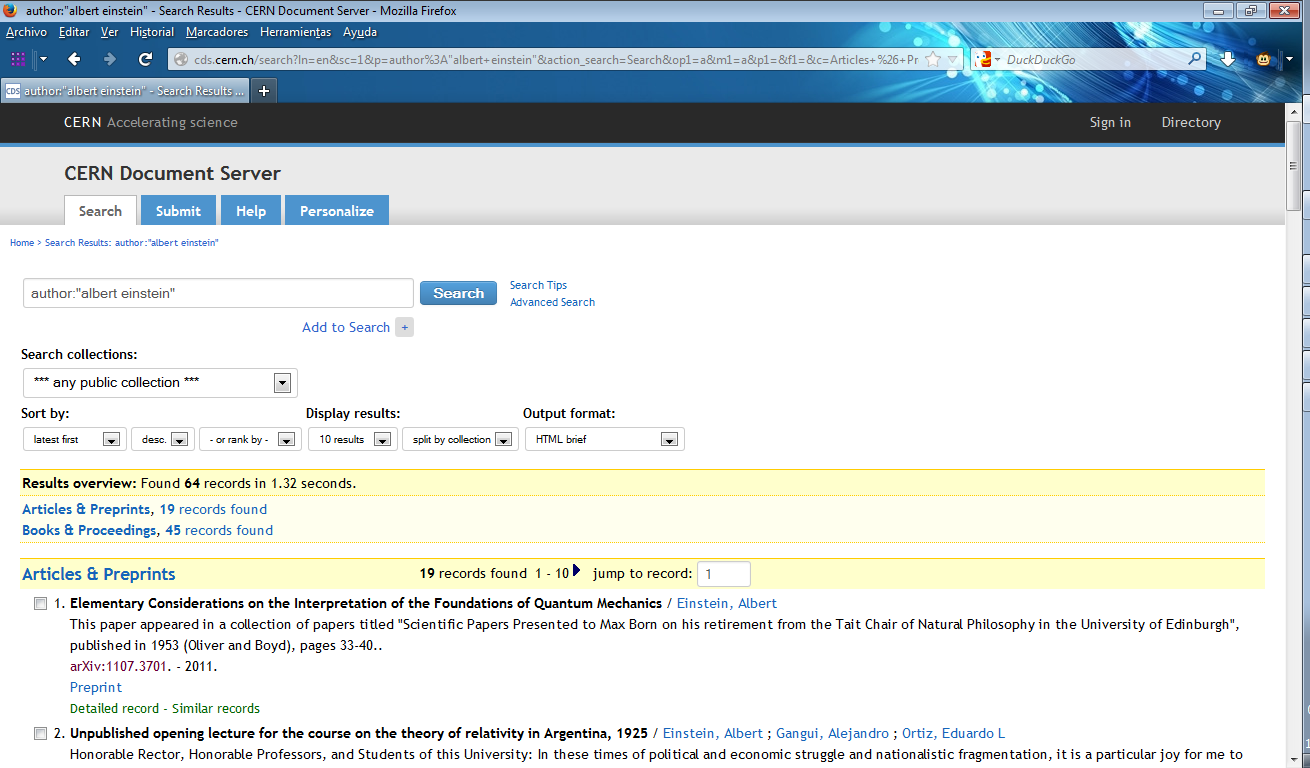
\includegraphics[height=7 cm]{figures/cds_screenshot.png}
\label{cds_screenshot}
\caption{CDS search result interface}
\end{figure}
 


Invenio\cite{invenio} is the software running behind CDS and is an open source project developed in parallel to CDS at CERN. Besides CDS, Invenio also supports around thirty scientific institutions worldwide including Fermilab, SLAC National Laboratory, INSPIRE and EPFL. 
Invenio is composed of several modules where each one can be mapped to a specific step in the workflow of a record. Figure \ref{invenio_architecture} presents the global architecture of Invenio. A detailed explanation of each module can be accessed in\cite{invenio_modules} 

\begin{figure}
\centering
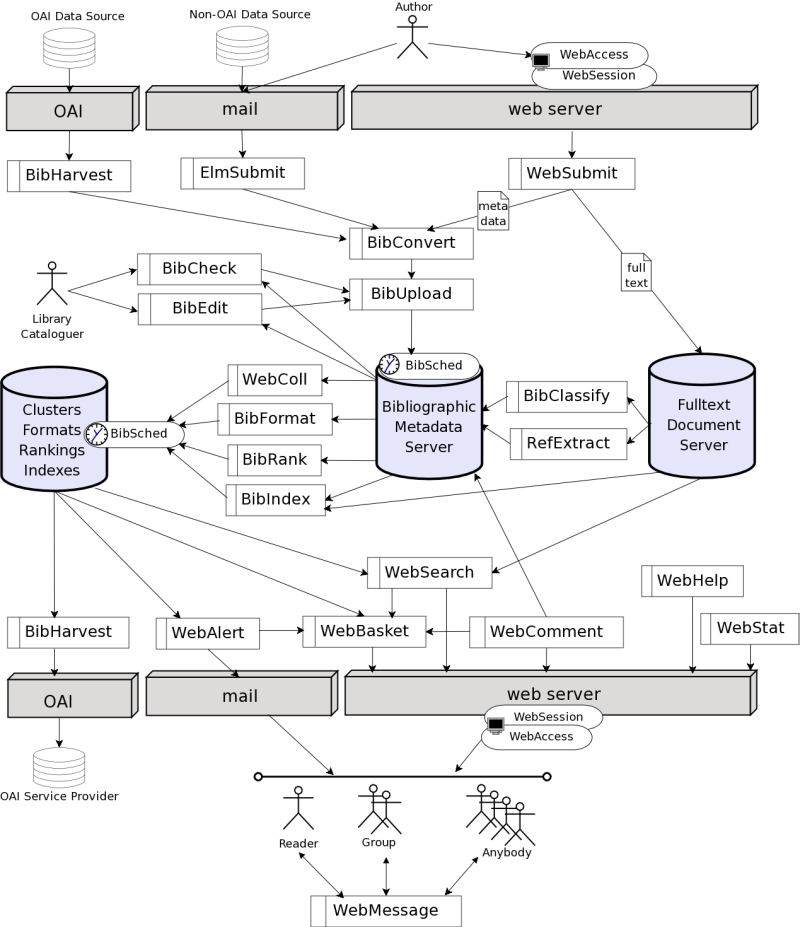
\includegraphics[height=10 cm]{figures/invenio.jpeg}
\label{invenio_architecture}
\caption{Invenio global architecture}
\end{figure}


\section{Project overview}
\subsection{Motivation}
The initial statement for this project was more generic and was encompassed as New ways to programmatically, accurately and efficiently extract data and metadata from digital files. During a first exploration around this topic, we focused our attention to the mathematical content that is stored in these files. After more discussions we identified that the extraction, storage, indexing and finally searching for mathematical content would be an and very useful project for CDS and an interesting research direction. CDS groups records in different categories or Collections such as Published Articles, Preprint, Photos, Books, General Talks among others. Some of these collections contain scientific documents in all of the different research areas where CERN is involved, and therefore a big amount of mathematical expressions are contained there. Only the Preprints collection contains 698581 records to the date, which harvest documents from services like ArXiV\cite{arxiv} where most of the documents are in the areas of physics, mathematics and statistics which are very rich in mathematical content.
Currently Invenio provides different ways of searching for records by specifying metadata fields like author:"Albert Einstein" or by keywords. However, there is no way to search for a given mathematical expression. The current workarounds would be to try to search for the name of the given expression if it is common enough to have been named like \emph{Schr\"oodinger equation}. This approach most of the times is not enough since most of the equations are not named and even named ones can be rewritten in several ways and each one may have a different importance to the user. This combination of factors, motivates the development of a complete system that allows users to search for relevant documents, based on mathematical expressions.

\subsection{Goals}

The specific goals of this project can be summarized as:

\begin{itemize}
\item Explore ways to automatically extract the mathematical content from a document collection
\item Investigate different approaches and formats to store mathematical expressions
\item Identify relevant features in a mathematical expression and how to use them to index equations
\item Using the created index, propose ways to efficiently retrieve relevant expressions and articles given an input query
\item Implement the previous steps into a complete system (A search engine) and integrate it into the Invenio software
\item Evaluate different approaches and the quality of the provided results
\item Identify deficiencies in our work and propose solutions and further direction on work
\end{itemize}

















